\section{Video Understanding Models}
\begin{frame}{}
    \LARGE Video Learning \& Generation: \textbf{Video Understanding Models}
\end{frame}

\begin{frame}[allowframebreaks]{Video Understanding Models}
    \begin{itemize}
        \item Video understanding involves analyzing and interpreting video data to extract meaningful information.
        \item Key tasks include:
        \begin{itemize}
            \item \textbf{Action recognition}: Identifying actions or activities in videos.
            \item \textbf{Object detection}: Locating and classifying objects within video frames.
            \item \textbf{Scene understanding}: Analyzing the context and environment in which actions occur.
            \item \textbf{Temporal analysis}: Understanding how actions evolve over time.
        \end{itemize}
    \end{itemize}
\framebreak
    \begin{figure}
        \centering
        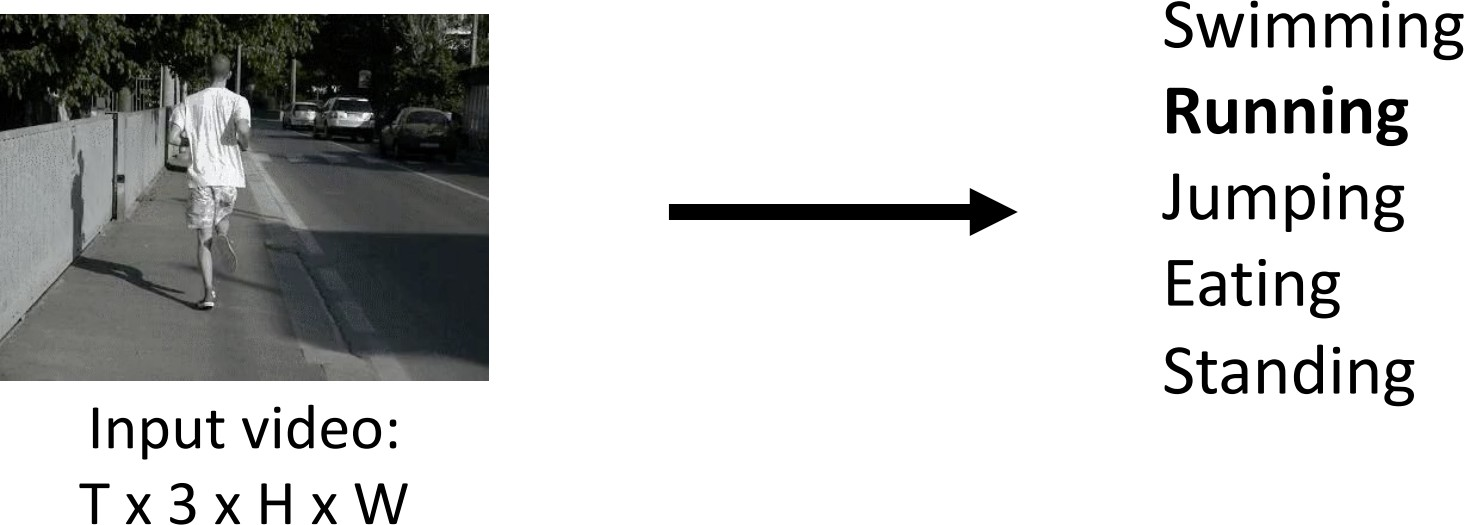
\includegraphics[width=1\textwidth,height=0.9\textheight,keepaspectratio]{images/video/slide_4_1_img.jpg}
    \end{figure}
\framebreak
    \begin{itemize}
        \item To understand videos, models need to look at both:
        \begin{itemize}
            \item What’s in each frame (spatial info).
            \item How things move or change (temporal info).
        \end{itemize}
        \item How do we do this?
        \begin{itemize}
            \item Use CNNs to spot patterns in images.
            \item Use RNNs or LSTMs to follow changes over time.
            \item Use 3D CNNs to look at several frames together.
            \item Use Transformers to connect information across the whole video.
        \end{itemize}
    \end{itemize}
\framebreak
    \begin{figure}
        \centering
        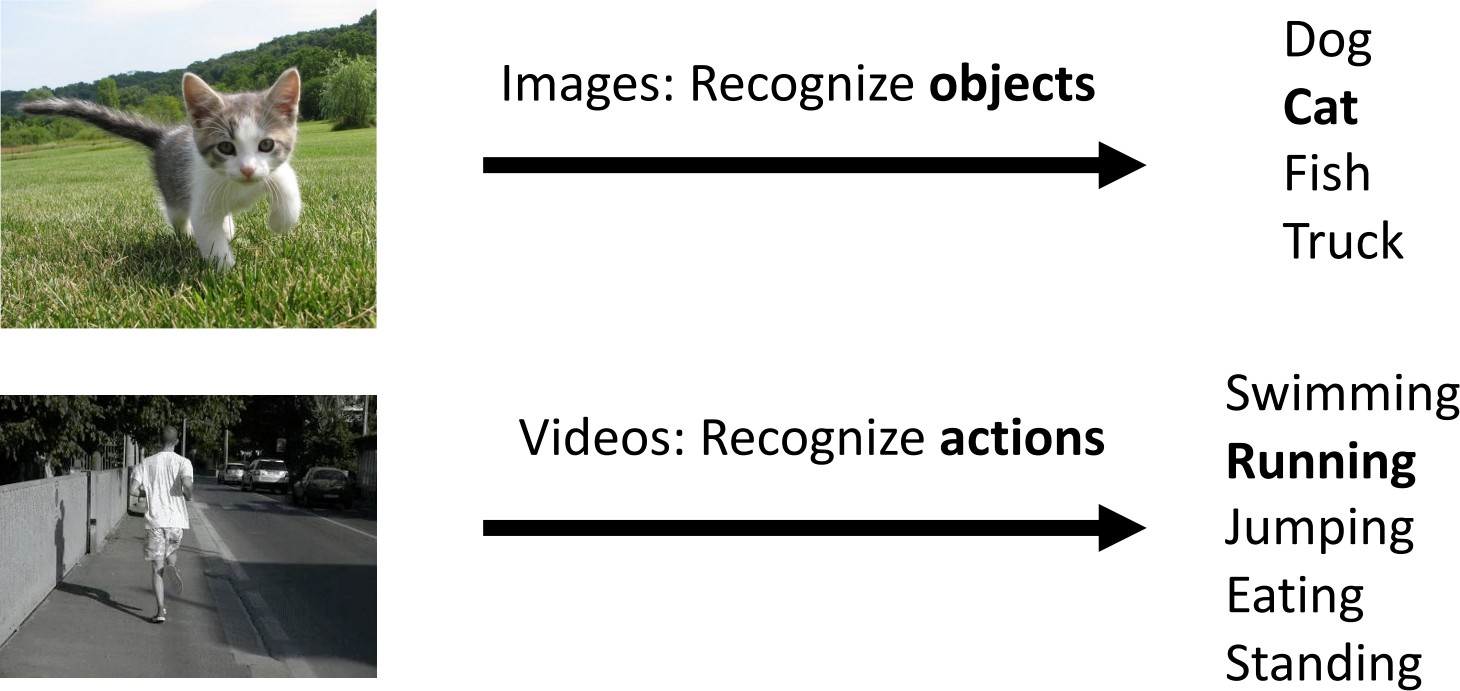
\includegraphics[width=1\textwidth,height=0.9\textheight,keepaspectratio]{images/video/slide_5_1_img.jpg}
    \end{figure}
\framebreak
    \begin{itemize}
        \item These models learn from lots of labeled videos.
        \item We check how well they work using accuracy, precision, recall, and F1-score.
        \item New research is making models faster, more reliable, and better at handling different types of videos.
        \item Where is this useful?
        \begin{itemize}
            \item Security and surveillance.
            \item Self-driving cars.
            \item Sports analysis.
            \item Healthcare monitoring.
            \item Recommending videos online.
        \end{itemize}
    \end{itemize}
\end{frame}

\subsection{Training on Clips}

\begin{frame}[allowframebreaks]{Training on Clips: Key Considerations}
    \begin{itemize}
        \item \textbf{Clip Length Selection:} Typically, short clips of 16--64 frames are used to balance computational cost and temporal coverage.
        \item \textbf{Batch Size vs. Temporal Context:} Increasing clip length provides more temporal context but reduces the possible batch size due to memory constraints.
        \item \textbf{Pretraining for Transfer Learning:} Models are often pretrained on large-scale video datasets (e.g., Kinetics, Sports-1M) to improve performance on downstream tasks.
    \end{itemize}
\framebreak
    \begin{figure}
        \centering
        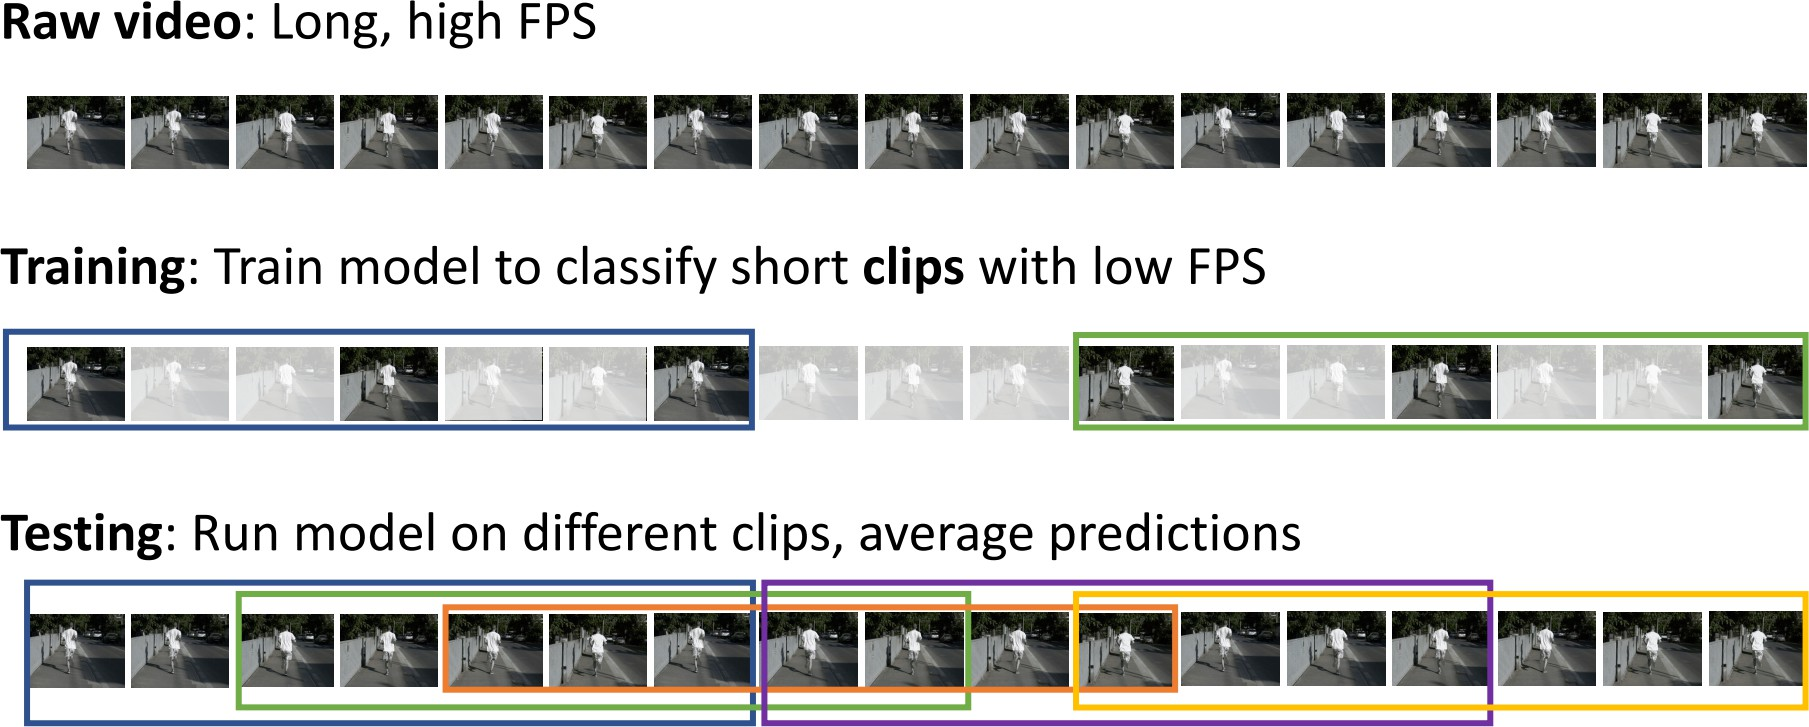
\includegraphics[width=1\textwidth,height=0.9\textheight,keepaspectratio]{images/video/slide_8_1_img.jpg}
    \end{figure}
\end{frame}
\subsection{Single Frame CNNs}

\begin{frame}[allowframebreaks]{Single-Frame CNN}
    \begin{itemize}
        \item Treat each frame independently
        \item Use pretrained ImageNet backbones
        \item Ignores temporal context; serves as a baseline
    \end{itemize}
\framebreak
    \begin{figure}
        \centering
        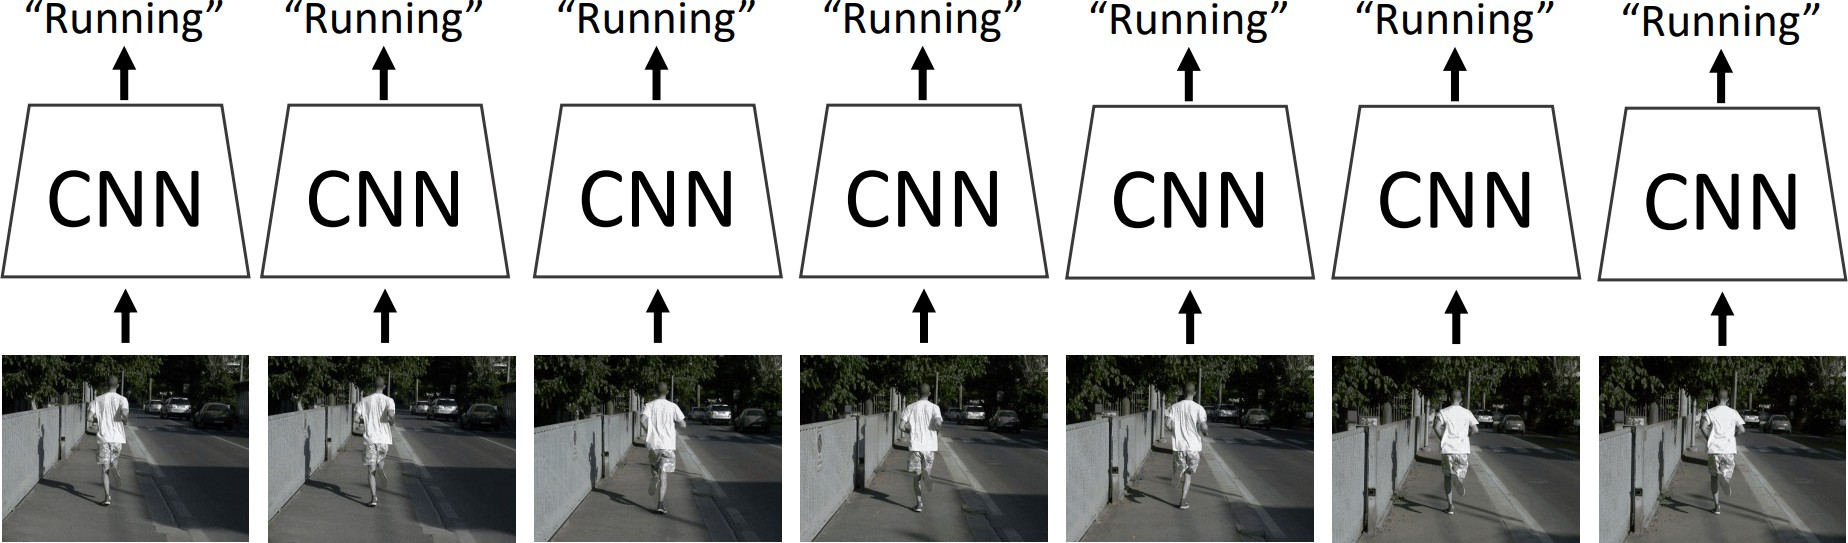
\includegraphics[width=1\textwidth,height=0.9\textheight,keepaspectratio]{images/video/slide_9_1_img.jpg}
    \end{figure}
\end{frame}
\subsection{Late Fusion}

\begin{frame}[allowframebreaks]{Late Fusion: Overview}
    \begin{itemize}
        \item \textbf{Process frames separately}, then combine their representations.
        \item \textbf{Fully Connected Fusion}: Concatenate frame features, then use fully connected (FC) layers.
        \item \textbf{Pooling Fusion}: Apply average or max pooling across time dimension.
    \end{itemize}
    \vspace{1em}
    \textbf{Pros:} Simple and easy to implement.\\
    \textbf{Cons:} Weak temporal modeling; ignores complex temporal dependencies.
\end{frame}

\begin{frame}[allowframebreaks]{Late Fusion (with FC layers)}
    \begin{figure}
        \centering
        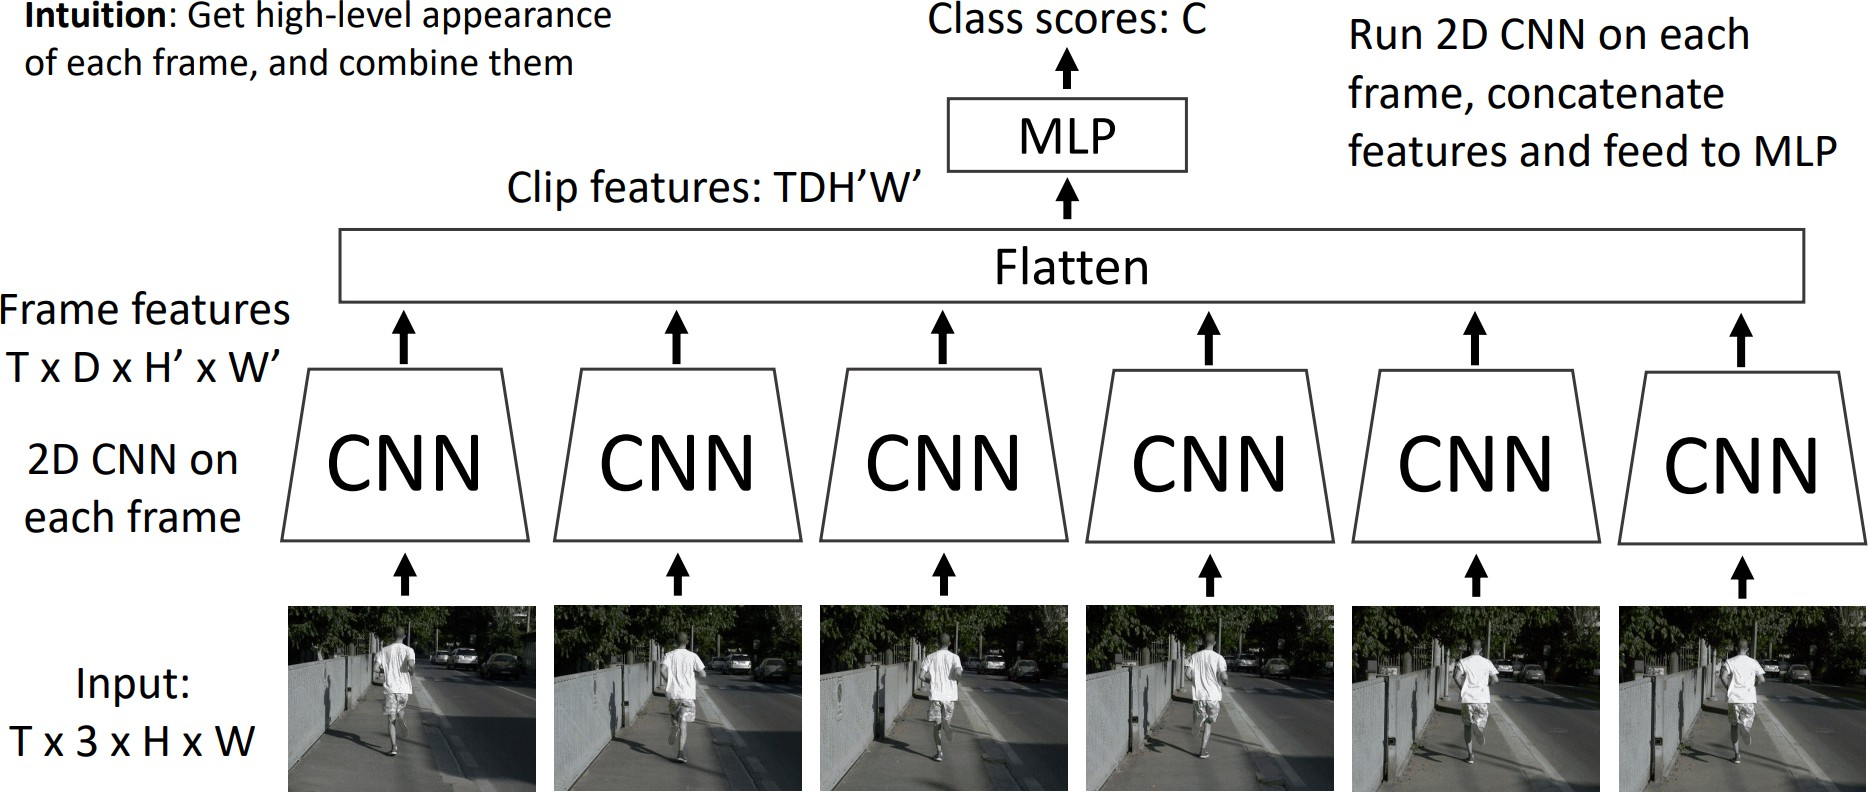
\includegraphics[width=1\textwidth,height=0.9\textheight,keepaspectratio]{images/video/slide_10_1_img.jpg}
    \end{figure}
\end{frame}

\begin{frame}[allowframebreaks]{Late Fusion (with pooling)}
    \begin{figure}
        \centering
        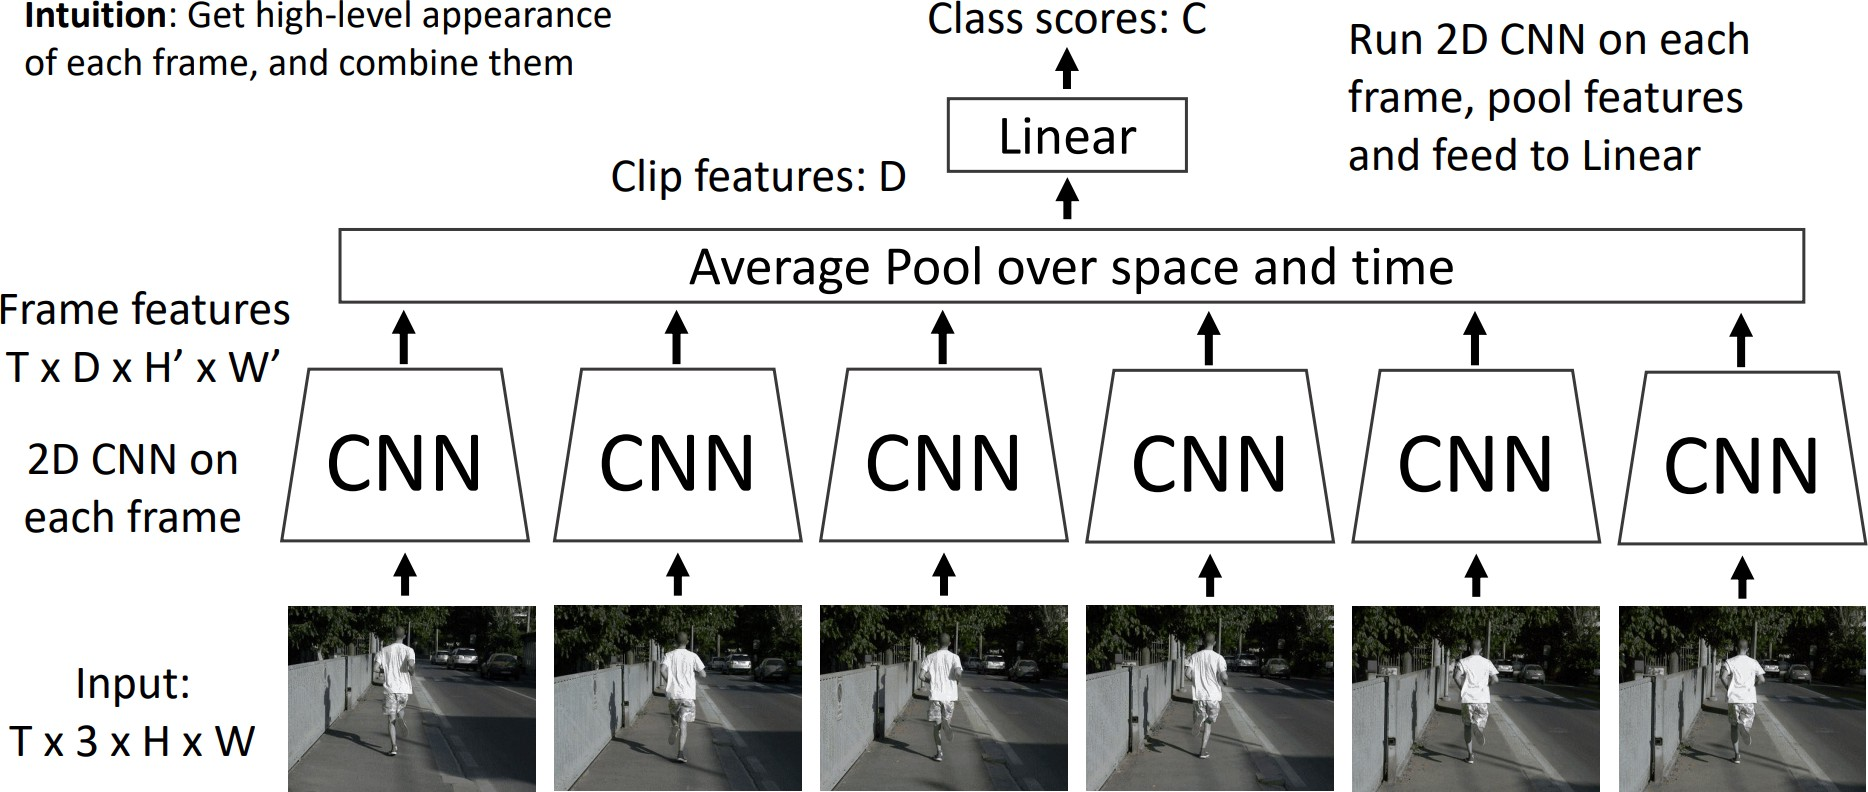
\includegraphics[width=1\textwidth,height=0.9\textheight,keepaspectratio]{images/video/slide_11_1_img.jpg}
    \end{figure}
\framebreak
    \begin{figure}
        \centering
        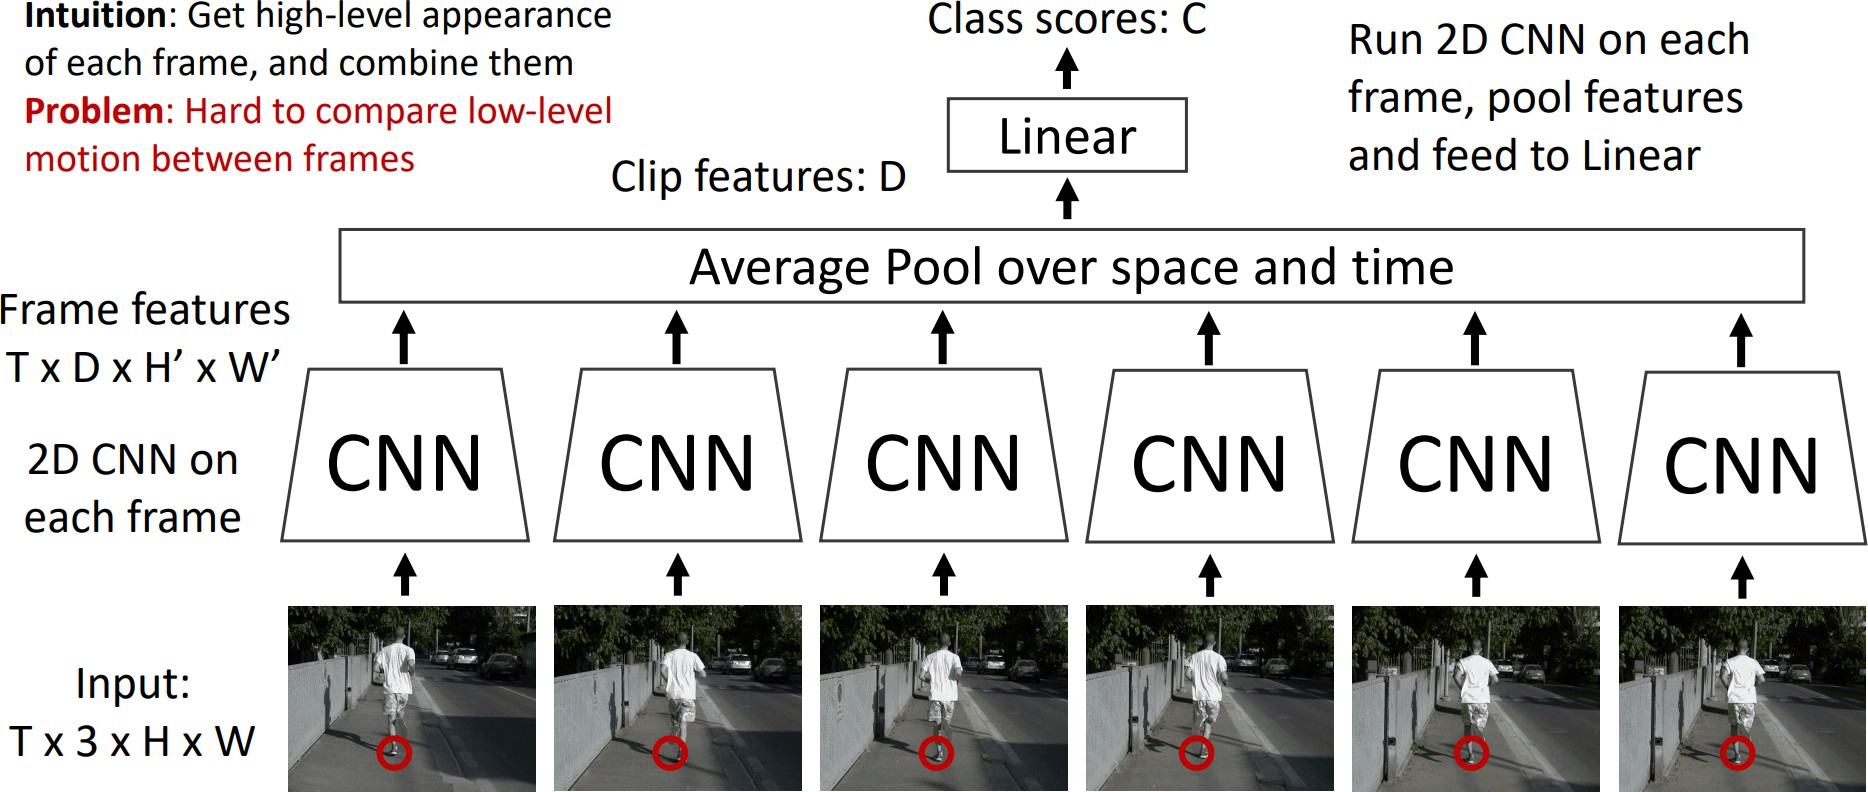
\includegraphics[width=1\textwidth,height=0.9\textheight,keepaspectratio]{images/video/slide_12_1_img.jpg}
    \end{figure}
\end{frame}
\subsection{Early Fusion}

\begin{frame}[allowframebreaks]{Early Fusion: Key Ideas}
    \begin{itemize}
        \item \textbf{Stack frames as input channels to 2D CNN}
        \item Learns short-term motion patterns
        \item Limited receptive field along time
    \end{itemize}
\framebreak
    \begin{figure}
        \centering
        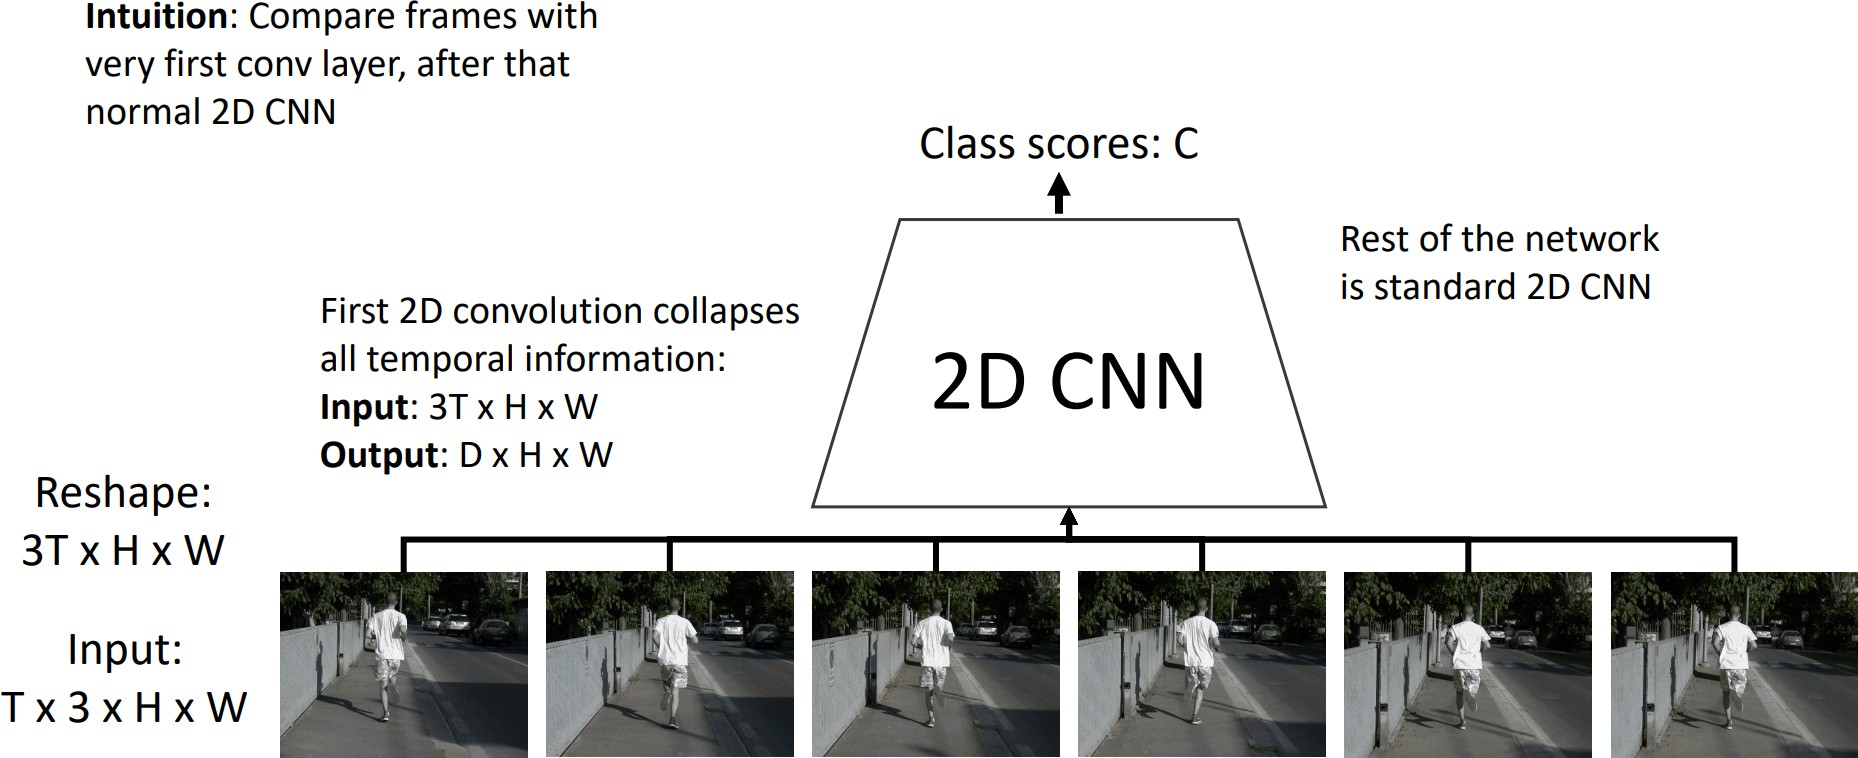
\includegraphics[width=1\textwidth,height=0.9\textheight,keepaspectratio]{images/video/slide_13_1_img.jpg}
    \end{figure}
\framebreak
    \begin{figure}
        \centering
        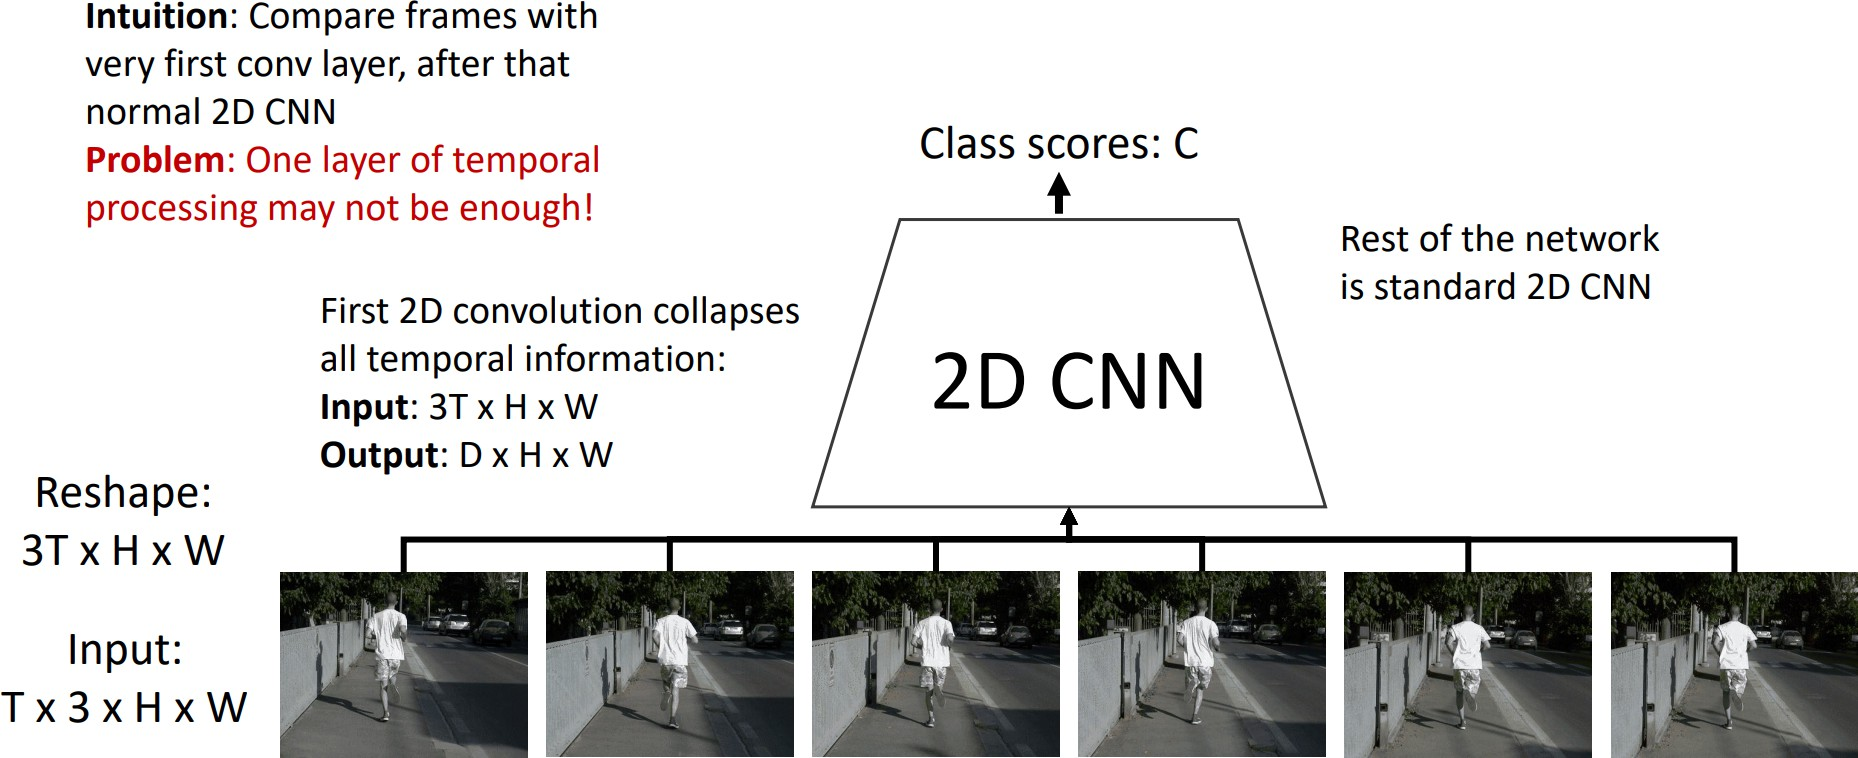
\includegraphics[width=1\textwidth,height=0.9\textheight,keepaspectratio]{images/video/slide_14_1_img.jpg}
    \end{figure}
\end{frame}
\subsection{3D CNN}

\begin{frame}[allowframebreaks]{3D CNN: Key Ideas}
    \begin{itemize}
        \item \textbf{3D Convolutional Networks}: Apply convolutional kernels across both spatial and temporal dimensions.
        \item \textbf{3D Kernels over Space-Time}: Filters operate on width, height, and time, enabling motion modeling.
        \item \textbf{Capture Local Spatio-Temporal Features}: Learn patterns that span multiple frames, such as movement or actions.
        \item \textbf{High Computational Cost}: Increased parameters and operations compared to 2D CNNs, leading to higher resource requirements.
    \end{itemize}
\framebreak
    \begin{figure}
        \centering
        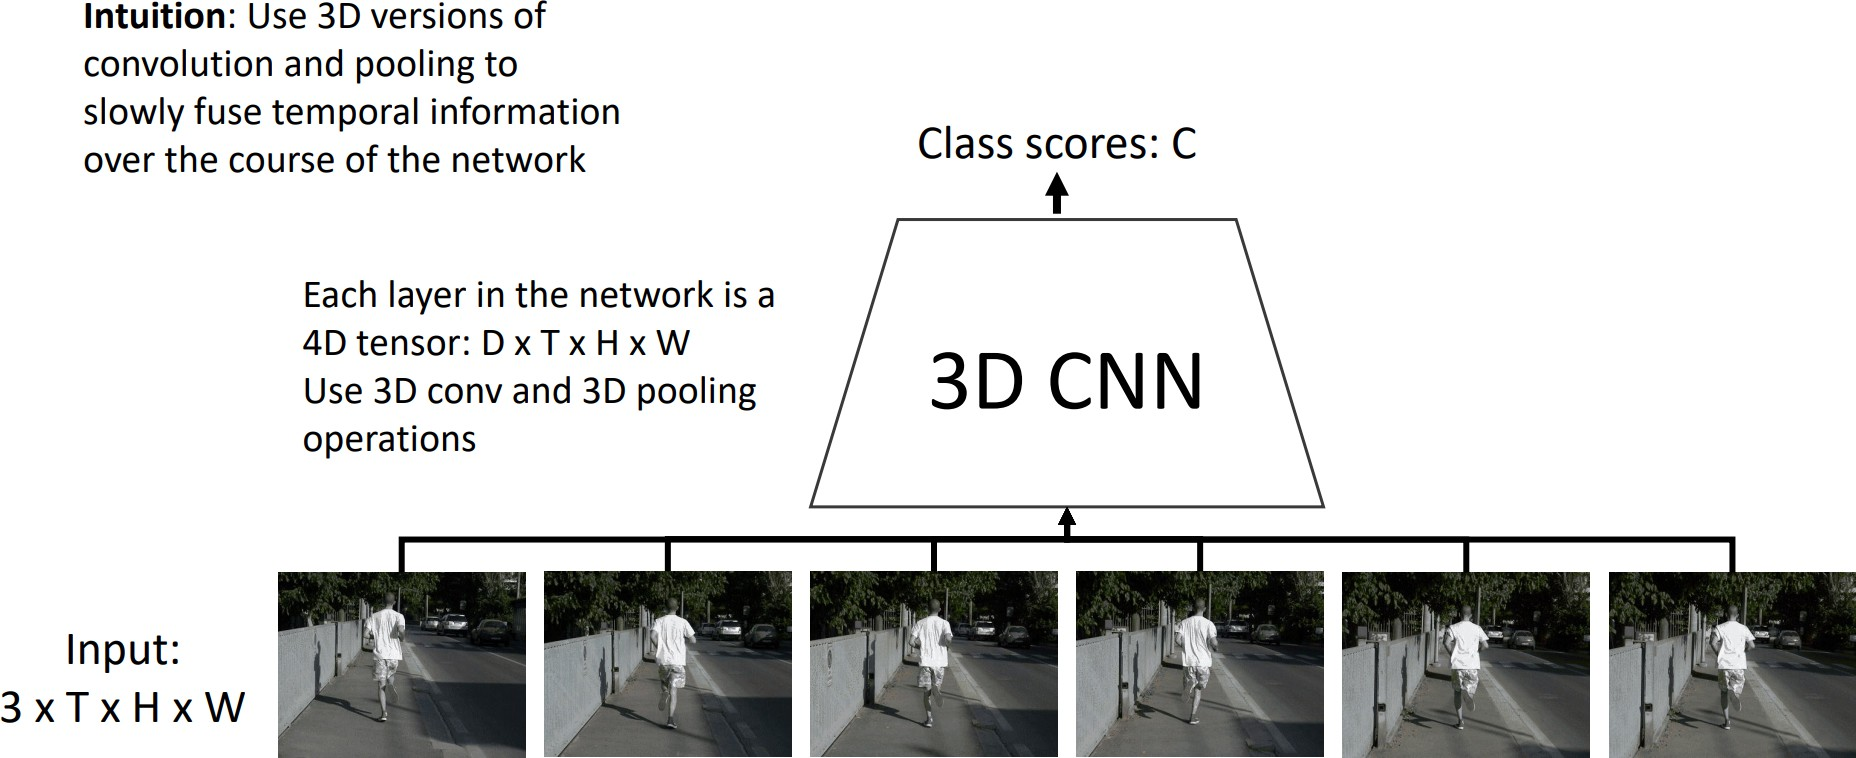
\includegraphics[width=1\textwidth,height=0.9\textheight,keepaspectratio]{images/video/slide_15_1_img.jpg}
    \end{figure}
\framebreak
    \begin{figure}
        \centering
        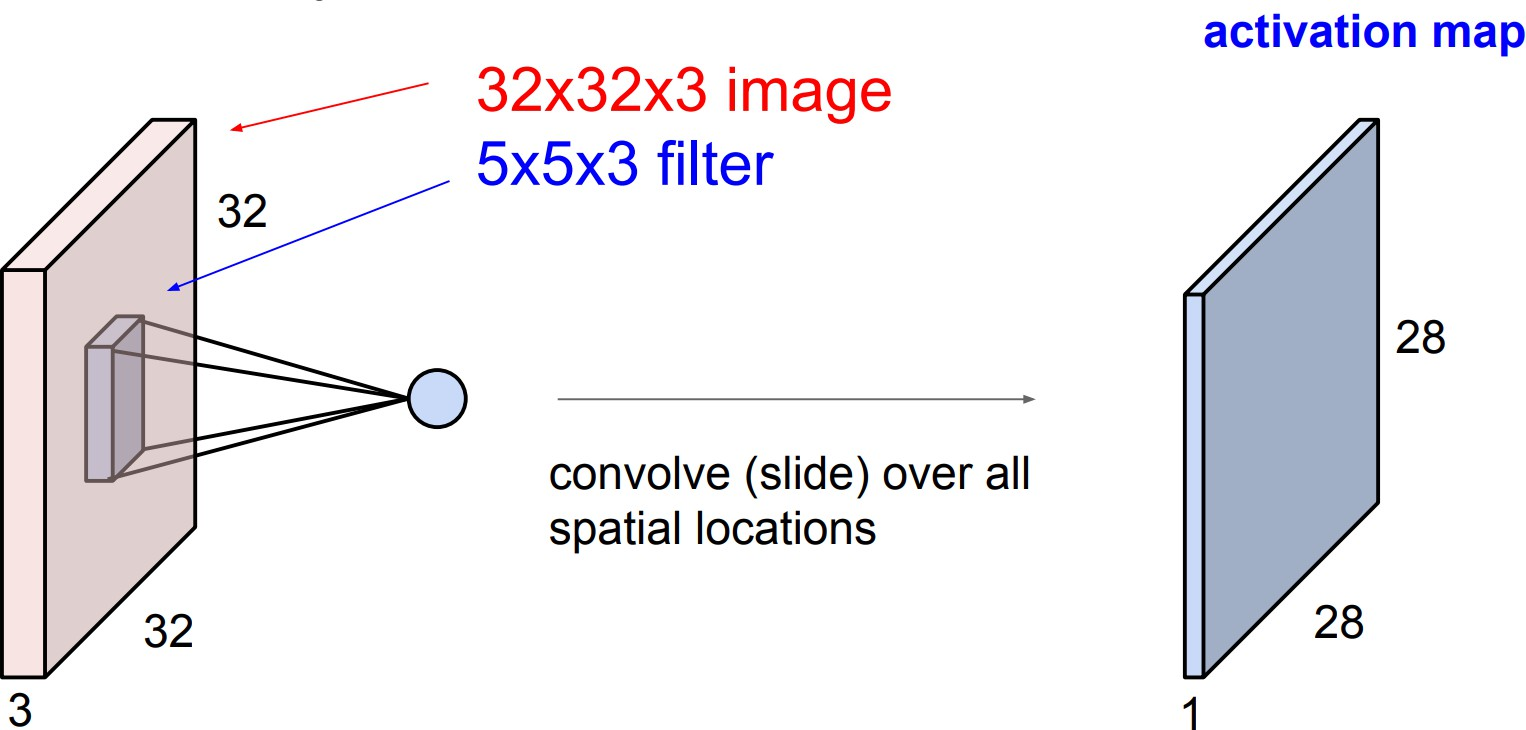
\includegraphics[width=1\textwidth,height=0.9\textheight,keepaspectratio]{images/video/slide_16_1_img.jpg}
    \end{figure}
\framebreak
    \begin{figure}
        \centering
        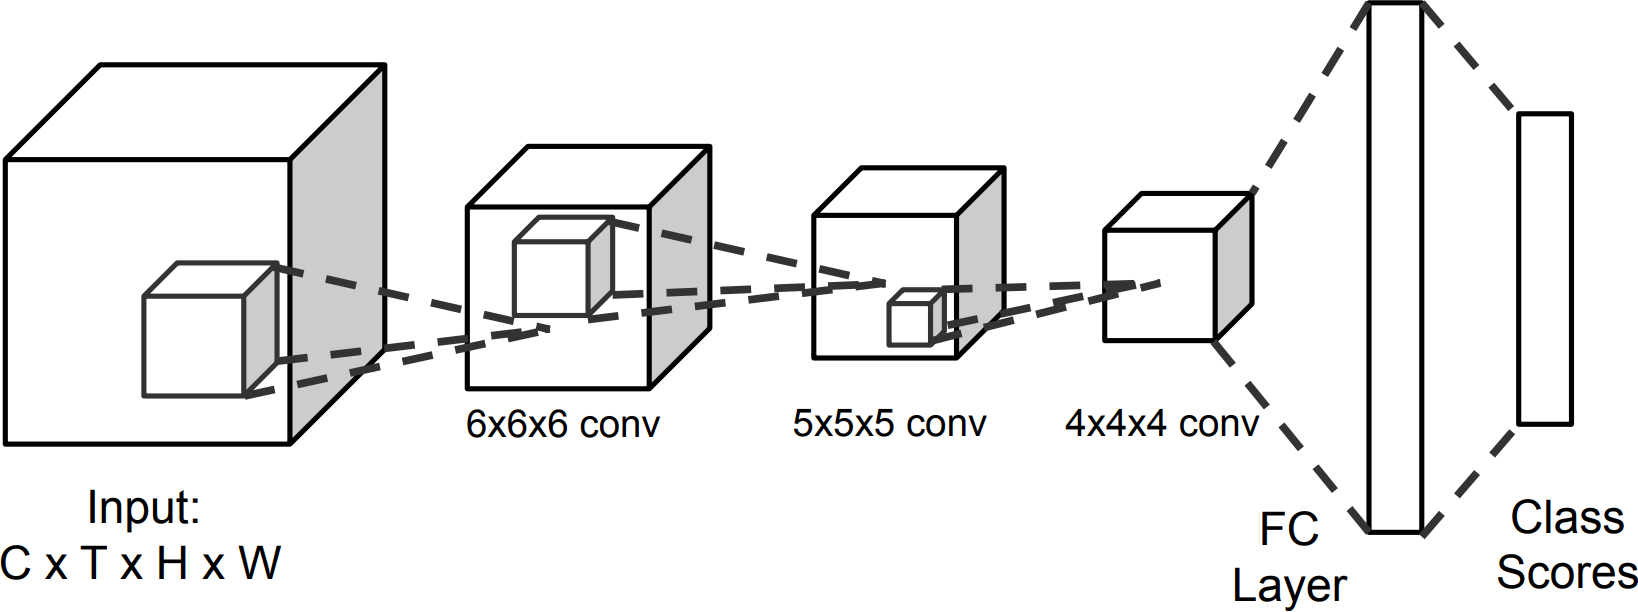
\includegraphics[width=1\textwidth,height=0.9\textheight,keepaspectratio]{images/video/slide_17_1_img.png}
    \end{figure}
\framebreak
    \begin{itemize}
        \item \textbf{3D CNNs} are powerful for video understanding, capturing both spatial and temporal features.
        \item They are particularly effective for tasks like action recognition, where understanding motion is crucial.
        \item However, they require significant computational resources and large datasets for training.
        \item \textbf{Applications}:
        \begin{itemize}
            \item Action recognition in videos.
            \item Gesture recognition.
            \item Video classification.
            \item Sports analysis.
        \end{itemize}
    \end{itemize}
\end{frame}
\subsection{C3D}

\begin{frame}[allowframebreaks]{C3D: Key Ideas}
    \textbf{Introduced by Tran et al., ICCV 2015}

    \begin{itemize}
        \item Uses $3 \times 3 \times 3$ convolutions on 16-frame video clips.
        \item Demonstrated strong performance on the UCF101 action recognition benchmark.
    \end{itemize}
    \begin{itemize}
        \item \textbf{3D Convolutional Networks}: Apply 3D convolutional kernels to capture spatio-temporal features.
        \item \textbf{Temporal Context}: C3D captures motion patterns by considering multiple frames simultaneously.
        \item \textbf{Pooling and Normalization}: Use pooling layers to reduce dimensionality and normalize features.
        \item \textbf{End-to-End Training}: Trained on large video datasets for tasks like action recognition.
    \end{itemize}
\framebreak
    \begin{columns}[T,onlytextwidth]
        \begin{column}{0.6\textwidth}
            \begin{itemize}
                \setlength{\itemsep}{1em}
                \item 3D CNN that uses all $3 \times 3 \times 3$ convolutions and $2 \times 2 \times 2$ pooling (except Pool1, which is $1 \times 2 \times 2$).
                \item Released model pretrained on Sports-1M: widely used as a video feature extractor.
                \item \textbf{Problem:} $3 \times 3 \times 3$ convolutions are very expensive!
                \begin{itemize}
                    \item AlexNet: 0.7 GFLOP
                    \item VGG-16: 13.6 GFLOP
                    \item C3D: 39.5 GFLOP (2.9$\times$ VGG!)
                \end{itemize}
            \end{itemize}
        \end{column}
        \begin{column}{0.35\textwidth}
            \begin{figure}
                \centering
                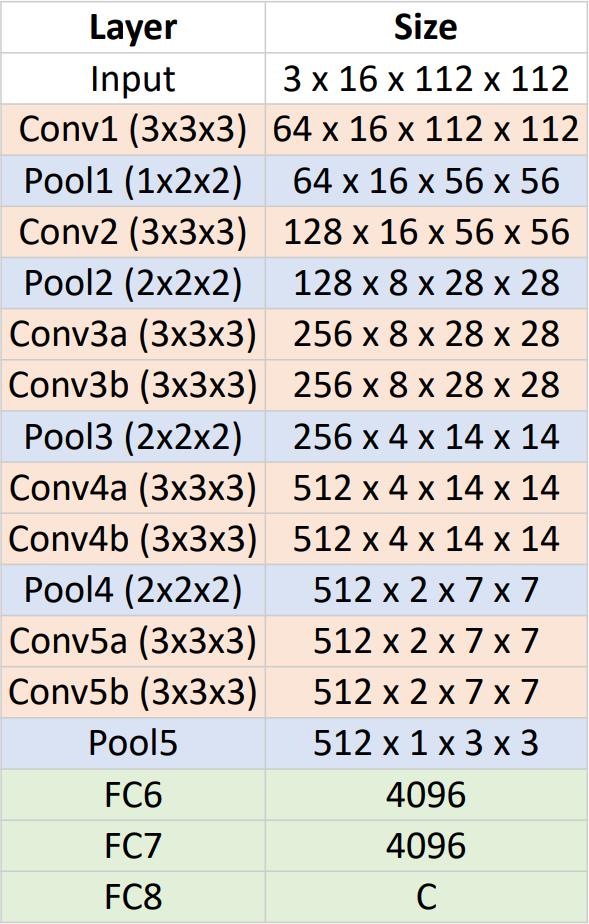
\includegraphics[width=\linewidth,keepaspectratio]{images/video/slide_19_1_img.png}
            \end{figure}
        \end{column}
    \end{columns}
\framebreak
    \begin{figure}
        \centering
        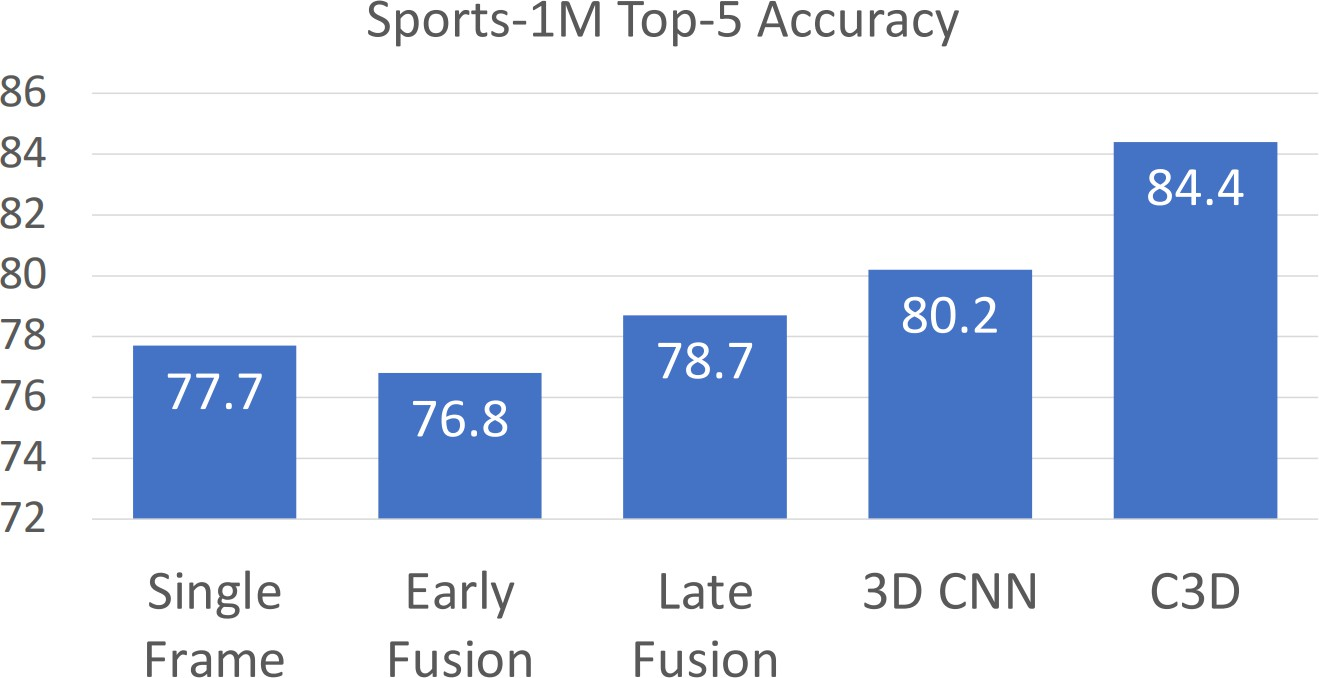
\includegraphics[width=1\textwidth,height=0.9\textheight,keepaspectratio]{images/video/slide_20_1_img.jpg}
    \end{figure}
\end{frame}